\cotefile{15}
\scanpage{87}
\mspage{VI.5}
$\mathrm{\handwritten{\rho}_{\overset{\handwritten{\sim}}{A}}:\overset{\handwritten{\sim}}{A} \handwritten{\longrightarrow} j_*j^*(\overset{\handwritten{\sim}}{A})}$ is an isomorphism, i.e. $\mathrm{j}$ satisfies condition (b)
of Section V as well as condition (a).

An important property of the integrally closed noetherian domain
$\mathrm{A}$ which will be invoked in several succeeding proofs is the following
theorem: if $\mathrm{M}$ and $\mathrm{N}$ are finitely generated $\mathrm{A}$-modules and there
is an isomorphism $\mathrm{f:M \handwritten{\longrightarrow} N}$ such that $\mathrm{f_{\handwritten{\mathfrak p}}:M_{\handwritten{\mathfrak p}} \handwritten{\longrightarrow} N_{\handwritten{\mathfrak p}}}$ is an
isomorphism for every $\mathrm{\handwritten{\mathfrak p}}$ in $\mathrm{P}$, then $\mathrm{f^{**}:M^{**} \handwritten{\longrightarrow} N^{**}}$ is an
isomorphism (where $\mathrm{M^{**}}$ is $\mathrm{\operatorname{Hom}_A(\operatorname{Hom}_A(M,A),A)}$, the double
dual of $\mathrm{M}$). A proof of this theorem can be found in (amongst other
sources) the thesis of the author, Chapter II, Lemma 0.1.

The following theorems will enable us to reinterpret the groups in
the exact sequence of Theorem V.12 in terms of algebras and modules
over $\mathrm{A}$.

THEOREM VI.5. Let $\mathrm{Y}$ be a subset of $\mathrm{X}$ containing $\mathrm{P}$.
Then if $\mathrm{\handwritten{\mathcal M}}$ is locally free of finite rank over $\mathrm{(Y,j^*(\overset{\handwritten{\sim}}{A}))}$, there is a
finitely generated reflexive module $\mathrm{N}$ such that $\mathrm{j^*(\overset{\handwritten{\sim}}{N}) \handwritten{\approx} \handwritten{\mathcal M}}$.

\uline{Proof:} We know that the finitely generated module
$\mathrm{N=\handwritten{\Gamma}(U,j_*(\handwritten{\mathcal M})\mid U)=\handwritten{\Gamma}(Y,\handwritten{\mathcal M})}$ has the property that $\mathrm{j^*(\overset{\handwritten{\sim}}{N}) \handwritten{\approx} \handwritten{\mathcal M}}$, where
$\mathrm{U}$, as defined in the proof of Theorem VI.1, is an open set containing
$\mathrm{Y}$. We will show that $\mathrm{N}$ is reflexive. Let $\mathrm{N^{**}=\operatorname{Hom}_A(\operatorname{Hom}_A(N,A),A)}$.
Then there is a homomorphism $\mathrm{\delta:N \handwritten{\longrightarrow} N^{**}}$, giving rise to the sheaf
% archive sheet number: 86

\scanpage{88}
Dans le cas où $\mathscr G$ est quelconque, on peut
définir cependant le \inserted{\unsure{lien|$L$}} $L'=\operatorname{corad}(L)$, qui est
commutatif, et il correspond à une
gerbe quotient $\mathscr G'$ de lien commutatif $L'$.
D'ailleurs, $L'$ correspond à un groupe
algébrique \inserted{$H$}, et ce qui précède prouve que
$(\operatorname{Ker}(\varepsilon:H\longrightarrow{}G_m))^{\unsure{\circ|0}}$ est un tore \uline{compact}.

\figure{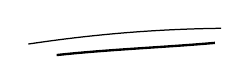
\begin{tikzpicture}
\draw[line width=.45pt] (0,0) .. controls (.8,.12) and (1.6,.19) .. (2.45,.20);
\draw[line width=.85pt] (.36,-.14) .. controls (1,-.07) and (1.75,-.04) .. (2.37,.015);
\end{tikzpicture}}

Nous envisageons maintenant une \deleted{gerbe}
catégorie de motifs munie d'un
\deleted{\unsure{automo|autre}} \unsure{hom|fonc|Frobenius} tensoriel dans \unsure{Abli-|Weil-|$\mathbb R$li-|Aut}$\unsure{\overline{\mathcal C}|\overline{=}}$
qui soit ``\unsure{génératrice|générateur}''. Ainsi $L$ est commutatif
et correspond à un groupe \deleted{\unsure{commutatif}}\inserted{\unsure{alg.}} \deleted{de type}
\deleted{\unsure{$G$}} multiplicatif $G$, \uline{muni} d'un
élément $f$ (``frobenius''), et $G$ est
engendré (au sens de Zariski) par
$f$. \deleted{Dans le cas qui nous occupe,}
\deleted{\unsure{Prenant le caractère|Prenant $L$ comme}\ \unsure{dessus}\unsure{,}}
\deleted{\unsure{soit|voit}}.
% archive sheet number: 87

\scanpage{89}
% Typescript inverted in the scan.
\uline{Remarque} 3.13. Voici une généralisation parfois utile de 3.5. b). Considérons
une partie $\mathrm{E}$ de $\mathrm{X}$ telle que pour tout morphisme étale $\mathrm{f:X'\quad X}$, $\mathrm{E'=f^{-1}(E)}$
soit ``très dense'' dans $\mathrm{X'}$ (EGA IV 10.1.3.)\deleted{\unsure{x}}, i.e. que pour tout $\mathrm{f}$ comme ci-dessus,
tout ouvert $\mathrm{U}$ de $\mathrm{X'}$ qui contient $\mathrm{E'}$ soit égal à $\mathrm{X'}$. Alors les foncteurs
fibres $\mathrm{F_{\bar x}}$ sur $\mathrm{X_{\text{ét}}}$, pour $\mathrm{x\quad E}$, forment déjà une ``famille conservative''
(et par suite les corollaires 3.6. , 3.7. et 3.8. restent valables
en se bornant à y choisir $\mathrm{x\quad E}$). Cela se voit immédiatement en reprenant la
démonstration donnée de 3.5. b). Le résultat précédent s'applique notamment
dans les siutations suivantes:

a) $\mathrm{X}$ est un préschéma de Ja\deleted{\unsure{v|x}}cobson (EGA IV 10.4.1.), par exemple localement
de type fini sur un corps, ou sur $\mathrm{\operatorname{Spec}(\underline{Z})}$, et $\mathrm{E}$ est l'ensemble des
points fermés de $\mathrm{X}$.

b) $\mathrm{X}$ est localement de type fini sur un préschéma $\mathrm{S}$, et $\mathrm{E}$ est l'ensemble
des points de $\mathrm{X}$ qui sont fermé dans leur fibre.

c) $\mathrm{X}$ est localement noethérien, et $\mathrm{E}$ est l'ensemble des $\mathrm{x\quad X}$ tels que
$\mathrm{\bar x}$ soit un ensemble fini (i.e. un schéma semi-local de dimension $\mathrm{\quad 1}$) cf
EGA IV 10.5.3. et \deleted{\unsure{1|l}}10.5.5.
% archive sheet number: 88

\scanpage{90}
\diagram{\begin{tikzcd}[ampersand replacement=\&,row sep=1pt,column sep=2pt]
\& \parbox[t]{.85\linewidth}{a) pro\deleted{\unsure{tore}}\inserted{groupe de t.m.} $T$ sur $Q$, avec $f\in T(Q)$ engendrant $T$ (Zar)}\\
\Updownarrow \& {}\\
\& \parbox[t]{.85\linewidth}{b) Sous-groupe \deleted{de} $M$ de $\bar Q^*$, stable par $\operatorname{Gal}(\bar Q/Q)$}\\
\unsure{\Vert|\Updownarrow} \& {}\\
\& \parbox[t]{.85\linewidth}{c) Sous-catégorie str. pleine $\mathcal M'$ de la catégorie des vectoriels sur $Q$ avec
automorphisme \inserted{semi-simple} [i.e. de la catégorie des $Q[X]$ modules
\inserted{semi-simples} de dim finie sur $Q$] stable par $\otimes$, $\oplus$, sous objet}
\end{tikzcd}}

\deleted{\unsure{$a)\Rightarrow b)$}} Soit donné un groupe de t.m. $T$, avec ``générateur''
$f\in T(Q)$, et soit donné $G_m\xrightarrow{j}T$, ce qui équivaut
à se donner $j^*:M\longrightarrow\mathbb Z$, \inserted{invariant par $\operatorname{Gal}(\bar Q/Q)$}, ou une \unsure{graduation}\ \inserted{fonctorielle} sur
les objets de $\mathcal M$. \deleted{\unsure{Si de plus, il existe un}}
\inserted{\unsure{i.e.} \deleted{\unsure{$\varepsilon^*$}\illegible{2}}}
i.e. soit donné un objet $\Lambda$ de $\mathcal M$ \inserted{de rang 1} de \unsure{poids|puissance|disons} \unsure{,}
\inserted{de $\varepsilon:T\longrightarrow G_m$, \deleted{tel que} $\varepsilon\circ j(\lambda)=\lambda^{\alpha}$,}
i.e. $j^*(\varepsilon^*)=\alpha$,
\inserted{i.e. $\Lambda$ de degré $\alpha$.}
\deleted{\unsure{Posons|Pour} $\unsure{\varepsilon^*|\varepsilon} \deleted{\unsure{(f)}}=q$}
\deleted{\unsure{et} \unsure{$q^*$} de $|\varepsilon(f)|$}
\margin{$q=\varepsilon^*=\varepsilon(f)\in M\cap Q^*$}
% circled margin note, at left of the overwriting

\diagram{\begin{tikzcd}[ampersand replacement=\&,row sep=1pt,column sep=2pt]
\& \parbox[t]{.84\linewidth}{a) $T^\circ/\operatorname{Im}j$ est compact.}\\
\Downarrow \& {}\\
\& \parbox[t]{.84\linewidth}{b) \inserted{$q>0$ et} Pour $\forall$ $m\in M$, on a $|m|=\deleted{\unsure{j(f)}}q^{j^*(m)/\alpha}$.}\\
\Updownarrow \& {}\\
\& \parbox[t]{.84\linewidth}{c) \inserted{$q>0$ et} Pour tout $(E,f)\in\mathcal M$, si $E$ est de degré $i$,
les valeurs propres de $f$ dans $E_{\mathrm C}$ sont de val. absolue $q^{i/\alpha}$.}
\end{tikzcd}}

En effet, les valeurs propres des \deleted{$(E,f)\in$\unsure{$f$|$\mathcal M$},} $f$, pour $(E,f)\in\mathcal M$
de degré $i$, sont les $m\in M$ avec $\unsure{j(m)|j^*(m)}=i$. Donc
\deleted{\unsure{b signifie que}} c) et b) sont équivalentes.

\deleted{[Ils impliquent a), car $T'=T^\circ/\operatorname{Im}j$ est un tore \deleted{\unsure{ayant}}
- \unsure{possédant} $f'$ ayant la vertu que pour \unsure{tte}
représentation dans un $E$, les valeurs propres de
$f'$ opérant sur $E_{\mathrm C}$ sont de val. abs. $1$. \deleted{\unsure{Or il nous}}
\inserted{Or pour un} tore opérant, \inserted{\unsure{de simple|de simple-}} un ss-groupe fermé de $\operatorname{GL}(E_{\mathrm C})$ \unsure{qui est}, \deleted{\unsure{un tel}} est
\deleted{\unsure{par conséquent, un tore de} $\operatorname{GL}$ \unsure{dont les} $^\circ$ \unsure{de} $\mathbb R$ \unsure{opérant}}
\deleted{\unsure{sur} $E_{\mathrm C}$ sont de val. absolue $1$.}
\inserted{cpt.} Comme $T'_{\mathbb R}$ est un ss-groupe fermé de ce
dernier, cqfd \unsure{précisément}.]}
% archive sheet number: 89

\scanpage{91}
% Typescript inverted in the scan.
\mspage{\handwritten{43}}
supposer $\mathrm{X}$ affine et qu'il existe un préschéma affine $\mathrm{X'_{\handwritten{1}}}$, de
présentation finie, quasi fini et fidèlement plat sur $\mathrm{X}$, et un
$\mathrm{X}$-morphisme $\mathrm{X'_{\handwritten{1}} \handwritten{\longrightarrow} X'}$, ce qui nous ramène au cas où $\mathrm{f}$ est quasi\handwritten{-}fini.
Quitte à localiser encore sur $\mathrm{X}$, au sens de la topologie étale
cette fois, on voit qu'il existera un ouvert $\mathrm{X'_{\handwritten{1}}}$ de $\mathrm{X'}$ tel que
$\mathrm{X'_{\handwritten{1}} \handwritten{\longrightarrow} X}$ soit fini et surjectif, ce qui nous ramène au cas où $\mathrm{f}$ est
fini et surjectif, déjà traité dans a).

9.4.4. Dans le cas d), on peut supposer (en se localisant sur $\mathrm{X}$)
que $\mathrm{X}$ est réduit à un seul point, et même contenu de 1.1. q\deleted{\unsure{g|y}}u'il est
spectre d'un corps $\mathrm{k}$, puis (quitte à remplacer $\mathrm{X'}$ par un ouvert
affine non vide) que $\mathrm{X'}$ est affine et à fortiori $\mathrm{f}$ est quasi compact
et quasi séparé. Mais alors il est encore vrai que $\mathrm{f_{\unsure{*|x}}}$ commute
\margin{\handwritten{$\mathrm{\uparrow}$}}
à tout changement de base $\mathrm{Y \handwritten{\longrightarrow} X}$, comme nous verrons ultérieurement.
De plus, $\mathrm{f}$ est universellement ouvert (EGA IV 2.4.9.) donc on
est s\handwritten{ous} les conditions de 9.1. , et le raisonnement de 9.4.1. s'applique
encore.

\handwritten{Ceci achève la démonstration de 9.4.}
% archive sheet number: 90

\scanpage{92}
\deleted{\unsure{Le|Je}} Montrons que a) implique c). Soit en
effet \deleted{\unsure{donc}} $E$ un vectoriel \deleted{\unsure{avec $T$|sur $Q$}}\inserted{``de degré $i$''} avec $T$ opérant.
\deleted{\unsure{Alors les opé|Alors les opérations de} \unsure{Donc} $T_{\mathbb R}$ opère sur $E_{\mathbb R}$, et comme
\unsure{c'est là la chose qui se passe}}
Alors $T_{\mathbb R}$ opère sur $E_{\mathbb R}$. Soit $U$ le plus
grand sous-tore compact de $T_{\mathbb R}$. Il résulte
aisément de l'hyp. a) que $T_{\mathbb R}^{\unsure{\circ|0}}=U_{\deleted{\unsure{R}}\mathbb R}\cdot S_{\mathbb R}$,
où $S=\operatorname{Im}j$, \deleted{\unsure{et}}\inserted{et $U\subset\operatorname{Ker}\varepsilon$.} \deleted{Donc} $f$ est de la forme
$u\,j(x)$, ou du moins il existe un entier \deleted{\unsure{$\nu$ tel que}}\inserted{$\nu>0$ \unsure{tq}}
que
\[
f^\nu=u\cdot j(x)\qquad u\in U(\mathbb R),\quad x\in\mathbb R^*
\]
Or $U$ étant compact, les valeurs propres de $\forall$
$u\in U(\mathbb R)$ sont de val absolue $1$, donc celles
de $f^\nu$ sont de val. absolues égales à celles
de $j(x)$, or $j(x)$ est la \deleted{\unsure{signature}}\unsure{l'hom.} \deleted{\unsure{de}} par
$x^i$ \unsure{,} \inserted{donc les val. propres de $f$ sont de val. abs. $x^{i/\nu}$.}
D'autre part $\deleted{\varepsilon(u)=0}\ \varepsilon\mid U=0$ donc
\[
\varepsilon(\unsure{f|f^\nu})^{\deleted{\unsure{\nu}}\nu}=\varepsilon(u)\,\varepsilon j(x)=\varepsilon j(x)=x^\alpha,\qquad
\text{donc}\quad x^{i/\nu}=\varepsilon(f)^{i/\alpha}=q^{i/\alpha},
\]
d'où la conclusion.

\margin{?}
\deleted{[NB. Evidemment b) et c) n'impliquent pas a), \unsure{pour aucune|pour mieux},
car il y a des sous-groupes libres de $Q^*$ de
rang $\geq 2$ \unsure{dans|donc}]}

D'autre part, on voit que a équivaut au
fait que $\mathcal M$ est (avec ses deux structures suppl.
provenant de $j,\varepsilon$) munissable d'une structure
``positive'' du style motivique. Ceci, d'autre part,
\unsure{via|par} un argument connu, implique que
% archive sheet number: 91

\scanpage{93}
% Typescript inverted in the scan.
\mspage{\handwritten{42}}
d'où un homomorphisme $\mathrm{f^{\unsure{*|x}}(G)\mathrel{\relbar\joinrel\handwritten{>}} F'}$ et ce dernier est evidemment
compatible avec les données de descente. Il reste à examiner si cet
homomorphisme est un \uline{isomorphisme.}
\figure{\begin{tikzpicture}[x=1cm,y=1cm]
\draw[line width=.35pt] (0,-.23) .. controls (-.09,-.18) and (-.02,.02) .. (.12,.05) .. controls (.6,.08) and (.79,.05) .. (1.2,.07) .. controls (1.65,.02) and (1.72,.13) .. (2.22,.14) -- (4.24,.18) .. controls (4.53,.18) and (4.59,.24) .. (4.56,.40) .. controls (4.56,.46) and (4.53,.49) .. (4.48,.49);
\end{tikzpicture}}
Noter que $\mathrm{G}$ est aussi définissable par l'exactitude de
\diagram{\begin{tikzcd}[ampersand replacement=\&,column sep=large]
\mathrm{G}\arrow[r,dash,"\handwritten{>}"{pos=1,anchor=east,inner sep=0pt}] \& \mathrm{f_*(F')}\arrow[r,dash,shift left=.6ex,"\handwritten{>}"{pos=1,anchor=east,inner sep=0pt}]\arrow[r,dash,shift right=.6ex,"\handwritten{>}"{pos=1,anchor=east,inner sep=0pt}] \& \mathrm{g_*(F'')}\text{,}
\end{tikzcd}}
donc pour tout changement de base $\mathrm{Y\overset{h}{\mathrel{\relbar\joinrel\handwritten{>}}}X}$ \uline{qui commute à la formation
de} $\mathrm{f_*(F')}$ \uline{et} $\mathrm{g_*(F'')}$\handwritten{,} $\mathrm{h^*(G)=G_Y}$ s'identifie au faisceau ``descendu''
de $\mathrm{F'_{Y'}}$ par $\mathrm{Y' \mathrel{\relbar\joinrel\handwritten{>}}Y}$, et bien entendu l'homomorphisme
$\mathrm{f_Y^*(G_Y)\mathrel{\relbar\joinrel\handwritten{>}}(F_Y)'}$ est celui déduit de $\mathrm{f^*(G)\mathrel{\relbar\joinrel\handwritten{>}}F'}$ par changement
de base. Or supposons que \uline{le changement de base} $\mathrm{f}$ ; $\mathrm{Y=X'\mathrel{\relbar\joinrel\handwritten{>}}X}$
\uline{commute à la formation de} $\mathrm{f_*(F')}$ \uline{et} $\mathrm{g_*(F'')}$\handwritten{,} et notons que comme
$\mathrm{Y'=X' \handwritten{\times}_X X'}$ a une section sur $\mathrm{Y'=X'}$, donc $\mathrm{Y'\mathrel{\relbar\joinrel\handwritten{>}}Y}$ est un
morphisme de descente \uline{effective} pour toute catégorie fibrée, en particulier
pour $\mathrm{\handwritten{\unsure{\mathfrak F|\mathcal F}}}$, il s'ensuit que $\mathrm{f_{\deleted{\unsure{X}}\handwritten{Y}}^*(G_{\deleted{\unsure{X}}\handwritten{Y}})\mathrel{\relbar\joinrel\handwritten{>}}(F_{\deleted{\unsure{X}}\handwritten{Y}})'}$ est un isomorphisme,
donc $\mathrm{f^*(G)\mathrel{\relbar\joinrel\handwritten{>}}F'}$ dévient un isomorphisme après changement de
base $\mathrm{Y'=X'\quad {}_X X'\mathrel{\relbar\joinrel\handwritten{>}}X'}$. Comme ce dernier à une section,
$\mathrm{f^*(G)\mathrel{\relbar\joinrel\handwritten{>}}F'}$ est un isomorphisme, donc la donnée de descente envisagée
sur $\mathrm{F'}$ est effective.

9.4.2. Ceci prouve le théorème 9.4. dans le cas a), grâce à 5.6.
Le cas b) résulte également du fait que si $\mathrm{f}$ est propre, alors $\mathrm{f_*}$
commute à \uline{tout} changement de base $\mathrm{Y' \mathrel{\relbar\joinrel\handwritten{>}} Y}$, (qui sera prouvé\unsure{'} dans un
exposé ultérieur).

9.4.3. Dans le cas c), la question étant locale sur $\mathrm{\unsure{Y|Y'}}$ on peut
% archive sheet number: 92

\scanpage{94}
$Q'$ : clôture \unsure{tot$^{\rm t}$|tot.} réelle de $Q$ ....

\margin{$\alpha=2$}
% circled
La condition a équivaut à la suivante, si $q\in Q^{* \unsure{-|{}}}$ est $>0$ :
\diagram{\begin{tikzcd}[ampersand replacement=\&,row sep=2pt]
\parbox[t]{.87\linewidth}{$\bigg\{$ \deleted{\unsure{on a $M$ \illegible{1}}}
\inserted{Pour tout $\lambda\in M$, $\exists$ \unsure{$r|m$}$>0$ tel que}
$\deleted{\unsure{\lambda}}\lambda^{r}\in Q'(i)^*$, et pour tout $\lambda\in M$, il existe un
entier $i$ tel que $|\lambda|=q^{i/2}$ i.e. $\lambda\bar\lambda=q^i$}\\
\Updownarrow\\
\parbox[t]{.87\linewidth}{$\bigg\{$ Pour tout $\lambda\in M$, \deleted{il existe} on a $|\lambda|=q^{j^*(\lambda)/2}$ i.e. $\lambda\bar\lambda=q^{j^*(\lambda)}$}
\end{tikzcd}}
\margin{N.B. Le $i$ en question alors est uniquement déterminé et n'est autre que $j^*(\lambda)$.}

\uline{Cor} Soit $\lambda\in\bar Q$, tel que \deleted{il existe $q\in Q^{\unsure{\times|*}+}$, avec}
\[
\lambda_\alpha\bar\lambda_\alpha=\lambda\bar\lambda\boxed{\in Q}
\quad\text{pour tout conjugué $\lambda_\alpha$ de $\lambda$. Alors $\exists\unsure{r|n}>0$,}
\]
\inserted{$\unsure{\Vert|=}\ q$}\quad \inserted{$|\lambda_\alpha|^2=|\lambda|^2$}
tel que $\lambda^{r}\in Q'(i)$, [donc la condition ne dépend pas du
plongt de $Q(\lambda)$ dans $\bar Q\subset\unsure{C|\mathbb C}$], et \unsure{.?.}
il existe $M,\varepsilon,j\ldots$ \inserted{relatifs à $f$} tel que $\lambda\in M$ (et \unsure{réciprt|vice versa}).

\margin{\uline{N.B.} Si un tel $\lambda$ est réel (donc tot réel !) on a $\lambda^2=q^i$ donc $\lambda=(q^{1/2})^i$, \uline{cas trivial}}
% slanted
\uline{Proposition} Soit $\lambda\in\bar Q^*$, et $q\in Q^{*+}$. Conditions équivalentes

(i) $\exists$ entier $i$ tel que pour $\forall$ conjugué $\lambda_\alpha$ de $\lambda$, on ait $|\lambda_\alpha|=q^{i/2}$
i.e. $\lambda_\alpha\bar\lambda_\alpha=q^i$

(ii bis) $\exists$ entier $n>0$ tel que $\lambda^n\in Q'(i)$, et \deleted{\unsure{$\exists i$|$\exists$}} entier $i$ tel que
$|\lambda|=q^{i/2}$ i.e. $\lambda\bar\lambda=q^i$ i.e. $\lambda^n\overline{\lambda^n}=q^{in}$

(ii) $\lambda\in Q'(i)$, il existe entier $i$ tel que $|\lambda|=q^{i/2}$, \unsure{id.|i.e.} $\lambda\bar\lambda=q^i$

(iii) $\exists$ un groupe de t.m. $G$ sur $Q$, et un élément $f$ de $G(Q)$,
$\deleted{\text{tel que l'on}}\ G_m\mathrel{\mathop{-}\limits^{j}}G\mathrel{\mathop{-}\limits^\varepsilon}G_m$, avec $\varepsilon j(\lambda)=\lambda^2$,
$\varepsilon(f)=q$, \inserted{avec et $\operatorname{Ker}\varepsilon$ compact}, tels que $\lambda$ soit une valeur propre de $f$
pour un $G$-Module de dim finie \inserted{sur $Q$} \unsure{convenable}, i.e.
$\lambda$ appartient à l'image de l'hom $M=D(G_{\bar Q})\longrightarrow\bar Q^*$
défini par $f$.

\margin{\deleted{NB. Les conditions \uline{n'impliquent pas} que $\lambda\in Q'(i)^*$, comme on voit p. ex. en prenant $\lambda=p^{1/4}$ ; Alors $Q(\lambda)$ n'est ni tot. imaginaire ($Q(p^{1/4})$ est réel) ni tot réel (car il est conjugué au $Q(\sqrt{\unsure{-p^{1/2}}})$ qui est \unsure{imaginaire}, donc n'est pas $\subset Q'(i)$}}
% slanted; crossed with long near-vertical strokes
(iv) Il existe une algèbre de Riemann commutative \deleted{\unsure{ab}}$A$ sur $Q$ et $f\in A^{\unsure{*|1|{}}}$
\inserted{et $i\in\mathbb N$, tels que $ff'=q^{i}$,}
et un hom $A\deleted{\unsure{C}}\longrightarrow\bar Q$, appliquant $f$ dans $\lambda$.
% archive sheet number: 93

\scanpage{95}
% Typescript inverted in the scan.
\mspage{-7-}
consequences of 1.9, of which only the following (cf. 1.7) will be stated
here, the paper comes to a close.

1.10 Theorem. \uline{Let} $\mathrm{k}$ \uline{be a perfect field of} $\mathrm{\dim\leq 1}$ \uline{and} $\mathrm{G}$ \uline{a
connected linear group over} $\mathrm{k}$. \uline{Then every conjugacy class over} $\mathrm{k}$ \uline{contains
an element over} $\mathrm{k}$.

After the remark that Kneser, using extensions of 1.8, has recently shown
(cf. 1.9) that $\mathrm{H^1(k,G)=0}$ if $\mathrm{k}$ is a $\mathrm{p}$-adic field and $\mathrm{G}$ a simply connected
semisimple group over $\mathrm{k}$, this introduction comes to a close.

\S2. \uline{Some recollections}. In this section we recall some known facts,
including some characterizations 2.11 of regular semisimple elements, and
establish some notations which are frequently used in the paper. If $\mathrm{k}$ is
a field, $\mathrm{k^*}$ is its multiplicative group. The term ``algebraic group'' is
often abbreviated to ``group''. If $\mathrm{G}$ is a group, $\mathrm{G_0}$ denotes its identity
component. If $\mathrm{x}$ is an element of $\mathrm{G}$, then $\mathrm{G_x}$ denotes the centralizer
of $\mathrm{x}$ in $\mathrm{G}$, and $\mathrm{x_s}$ and $\mathrm{x_u}$ denote the semisimple and unipotent parts
of $\mathrm{x}$ when $\mathrm{G}$ is linear. Assume now that $\mathrm{G}$ is a semisimple group, that
is, $\mathrm{G}$ is a connected linear group with no nontrivial connected solvable
normal subgroup. We write $\mathrm{r}$ for the rank of $\mathrm{G}$. Assume further that $\mathrm{T}$
is a maximal torus in $\mathrm{G}$ and that an ordering of the (discrete) character
group of $\mathrm{T}$ has been chosen. We write $\mathrm{\Sigma}$ for the system of roots relative
to $\mathrm{T}$ and $\mathrm{X_\alpha}$ for the subgroup corresponding to the root $\mathrm{\alpha}$.

2.1 $\mathrm{X_\alpha}$ \uline{is unipotent and isomorphic (as an algebraic group) to the}
% archive sheet number: 94

\scanpage{96}
\uline{Prop} Soit $K$ un corps de nbs fini sur $Q$,
$L$ une extension quadratique de $K$, $p_0$ un idéal
premier de $K$, \deleted{$p,p'$} qui se décompose dans $L$ dans
deux idéaux premiers distincts $p,p'$. Alors il
existe un $x\in L^*$ \deleted{dont le diviseur \unsure{absolu} soit}
\deleted{tel que} dont le diviseur \deleted{soit} $h(p-p')$, \inserted{où $h\in\mathbb N^*$,} et tel que
\deleted{\unsure{Alors}} $x\,\sigma x=1$, où $\sigma$ est l'autom non trivial de $L/K$.
\margin{Plus précisément, à torsion près les diviseurs des éléments de $L$ tels que $N_{L/K}x=1$, sont les diviseurs de $L$ de norme $1$ !}
% slanted

En effet, \deleted{\unsure{comme le groupe des}}\inserted{si $h$ est l'ordre} du groupe de
classes \inserted{de div.} de $L$, il existe un $y$ de diviseur
$h(p-p')$. Alors $y\,\sigma y$ est un élément de $K$ dont le
diviseur est \unsure{évidemt|évidemment} nul, donc c'est une unité $u$.
Donc si $z=y^2$, alors $\deleted{\unsure{x\bar x=}}\ \deleted{\unsure{x\bar x}}\ z\cdot\unsure{{}^{\sigma}z|\bar z}=(y\cdot{}^\sigma y)^2=u^2$,
donc si $x=\frac zu=\frac{y^2}{Ny}$, on aura $\operatorname{div}x=\operatorname{div}z=2\operatorname{div}y$
$=2h(p-p')$, et $x\,{}^\sigma x=(z\,{}^\sigma z)/u^2=1$.

\uline{N.B.} Supposons que $K$ \unsure{ext.|est} tot. réelle \deleted{\unsure{et $L$ une}}
\deleted{\unsure{extension de $Q$,|galoisienne de $Q$,}} \deleted{\unsure{telle que}} ext. quadratique
\deleted{\unsure{de $K$|et $K$}} tot. imaginaire \inserted{de $K$, supposée \uline{galoisienne} sur $Q$,}
. Soit $p$ un nb premier, et
$p_0$ idéal de $K$ au dessus de $p$, supposons que $\unsure{p_0|p}$ il n'y ait
qu'un \uline{seul idéal} \inserted{premier} $p$ \deleted{\unsure{p}} de $L$ sur $K$. Soit $\lambda$ un
\uline{entier} de $L$ tel que $\lambda\bar\lambda=p^i$. Alors $\lambda^2\bar\lambda^2=p^{2i}$ donc
si $\mu=\lambda^2/p^i=\frac{\lambda^2}{N_{L/K}\lambda}$ on aura $\mu\bar\mu=1$, \deleted{et $\mu$ est une unité en}
qui implique que $\mu$ est une unité en $p$, donc ($K$ étant galoisien)
en $\forall$ idéal premier au dessus de $p$ par le \unsure{raisonnt} (l'hyp. sur
$p$ \deleted{\unsure{donc}} \unsure{encore} \deleted{\unsure{avec}} \unsure{vraie} pour les $p'$), donc $\mu$ est une unité (NB. $\lambda$ \unsure{hors} $p$ est une
une racine de l'unité. Donc $\lambda=p^{i/2}u$, $u$ racine
de l'unité !
% archive sheet number: 95

\scanpage{97}
% Typescript inverted in the scan.
\mspage{-5-}
for $\mathrm{L}$, but there does not seem to be any simple way of relating 1.4 and
1.5 to their analogues for $\mathrm{L}$.

We now introduce a perfect subfield $\mathrm{k}$ of $\mathrm{K}$, although it appears
from recent results of A. Grothendieck on semisimple groups over arbitrary
fields that the assumption of perfectness is unnecessary for most of what
follows.

1.6 Theorem. \uline{Let} $\mathrm{G}$ \uline{be over} $\mathrm{k}$, \uline{and assume either that} $\mathrm{G}$ \uline{splits
over} $\mathrm{k}$ \uline{or that} $\mathrm{G}$ \uline{contains a Borel subgroup over} $\mathrm{k}$ \uline{but no component of
type} $\mathrm{A_n}$ ($\mathrm{n}$ \uline{even}). \uline{Then the set} $\mathrm{N}$ \uline{of} 1.4 \uline{can be constructed over} $\mathrm{k}$
(\uline{by appropriate choice of} $\mathrm{T}$, $\mathrm{\sigma_i}$, \uline{etc}.).

Together with 1.4 this implies that if $\mathrm{G}$ is simply connected in 1.6
the natural map from the set of regular elements over $\mathrm{k}$ to the set of
regular classes over $\mathrm{k}$ is surjective. For a group of type $\mathrm{A_n}$ ($\mathrm{n}$ even)
we have a substitute (see 9.7) for 1.6 which enables us to show:

1.7 Theorem. \uline{Assume that} $\mathrm{G}$ \uline{is simply connected and over} $\mathrm{k}$ \uline{and
that} $\mathrm{G}$ \uline{contains a Borel subgroup over} \unsure{.|,} $\mathrm{k}$. \uline{Then the natural map from the
set of semisimple elements over} $\mathrm{k}$ \uline{to the set of semisimple classes over} $\mathrm{k}$
\uline{is surjective. In other words, each semisimple class over} $\mathrm{k}$ \uline{contains an
element over} $\mathrm{k}$.

Theorems 1.6 and 1.7 are proved in \S9 where it is also shown (see 9.1
and 9.10) that the assumption that $\mathrm{G}$ contains a Borel subgroup over $\mathrm{k}$ is
essential.
% archive sheet number: 96

\scanpage{98}
Soit $K$ une extension \deleted{\unsure{gal}} \unsure{tot|tot.} réelle finie de $Q$,
$L$ ext. quadratique tot. imaginaire de $K$,
$q=p^{\unsure{n|-}}$ une puissance de nb premier. On cherche
les $\lambda\in K$ \uline{entiers} tels que $\lambda\bar\lambda=q^i$, i.e.
$|\lambda|=q^{i/2}$, \inserted{pour $i$ convenable $\in\mathbb N$.} Ce sont des unités exc. $p$, et
ils engendrent \deleted{le groupe des} un sous-groupe du
groupe \deleted{\unsure{$\forall$} des unités exc. $p$, \unsure{Soit les $\lambda$ entiers}}
formé des $\lambda$ unités exc. $p$ tels que
$\lambda\bar\lambda=q^i$ ($i\in\mathbb Z$). Notons que \deleted{ce sont des
unités \uline{absolues} exc. $p$. Donc finalement il en est
ces $\lambda$ s'écrivent $q^{i/2}u$, avec $u$} si $q$ est un
carré de \deleted{\unsure{$Q$|$K$}}$K$, on peut écrire un $\lambda$
sous la forme $\lambda=q^{i/2}u$, où $u$ est une unité
exc. $p$ telle que $u\bar u=1$, \unsure{Ce|En} qui implique que
$u$ est une \uline{unité absolue} exc. $p$. Les $u$ forment
un groupe $U$, et l'hom
\[
U\unsure{\longrightarrow|-}\mathbb Z^P
\qquad u\unsure{\mapsto|\sim}\bigl(v_{\mathfrak p}\unsure{(u)|N(u)}\bigr)_{\mathfrak p\in P}
\]
(où $P$ désigne l'ens des $\mathfrak p$ de $L$ sur $p$) est
de noyau fini. D'après la prop. plus haut,
son image est \inserted{\unsure{contenue} et} d'indice fini \unsure{du|dans} $\mathbb Z^{\deleted{\unsure{Q}}P'}$, où
\deleted{$P'$ est l'ens des $\mathfrak p$} formé des diviseurs de trace
\inserted{(rel. à $K$)} nulle. Donc si pour $\forall$ $\mathfrak p_0$ \deleted{\unsure{$\in$}\illegible{1}} idéal premier de
$K$ sur $p$ qui \uline{\unsure{splitte|splitt} en deux} dans $L$, on choisit
un $\mathfrak p$ au dessus, on trouve un isom à un
groupe fini près $U\simeq\mathbb Z^Q$, $Q$ étant \unsure{l'ens|l'un} des $\mathfrak p_0$
% archive sheet number: 97

\scanpage{99}
% Typescript inverted in the scan.
\mspage{-4-}
\uline{of regular classes of} $\mathrm{G}$.

In 7.4 an example of $\mathrm{N}$ is given: in case $\mathrm{G}$ is of type $\mathrm{\operatorname{SL}(r+1)}$
we obtain one of the classical normal forms under conjugacy. This special
case suggests the problem of extending the normal form $\mathrm{N}$ from regular
elements to arbitrary elements. In 7.1 it is shown that $\mathrm{N}$ is a closed
irreducible subset of $\mathrm{G}$, isomorphic as a variety to affine $\mathrm{r}$-space $\mathrm{V}$,
and in 7.9 (this is the main lemma concerning $\mathrm{N}$) that if $\mathrm{G}$ is simply
connected and $\mathrm{\chi_i}$ $\mathrm{(1\leq i\leq r)}$ denote the fundamental characters of $\mathrm{G}$
then the map $\mathrm{x\to(\chi_1(x),\chi_2(x),\ldots,\chi_r(x))}$ induces an isomorphism of $\mathrm{N}$
on $\mathrm{V}$. Then in \S8 the proof of 1.4 is given and simultaneously the following
important criterion for regularity is obtained.

1.5 Theorem. \uline{If} $\mathrm{G}$ \uline{is simply connected, the element} $\mathrm{x}$ \uline{is regular
if and only if the differentials} $\mathrm{d\chi_i}$ \uline{are independent at} $\mathrm{x}$.

At this point some words about recent work of B. Kostant are in order.
In [3] and [4] he has proved, among other thing, the analogues of our above
discussed results that are obtained by replacing the semisimple group $\mathrm{G}$ by
a semisimple Lie algebra $\mathrm{L}$ over the complex field (any algebraically
closed field of characteristic $\mathrm{0}$ will serve as well) and the characters
$\mathrm{\chi_i}$ of $\mathrm{G}$ by the basic polynomial invariants $\mathrm{u_i}$ of $\mathrm{L}$. The $\mathrm{\chi_i}$ turn
out to be considerably more tractable than the $\mathrm{u_i}$. Thus the proofs for $\mathrm{G}$
with no restriction on the characteristic are simpler than those for $\mathrm{L}$ in
characteristic $\mathrm{0}$. Assuming both $\mathrm{G}$ and $\mathrm{L}$ are in characteristic $\mathrm{0}$,
substantial parts of 1.1, 1.2, and 1.3 can be derived from their analogues
% archive sheet number: 98

\scanpage{100}
Conditions nécessaires pour qu'un $\lambda\in\bar Q$ soit valeur
propre de \deleted{\unsure{son|un}} frobenius, pour une variété projective
lisse définie sur le corps $\mathbb F_q$, $q=p^n$ :

\deleted{\[\left\{\begin{aligned}
&1)\ \lambda\in Q'(i)\\
&2)\ \deleted{\unsure{\lambda}}\lambda^2\ \text{est de la forme }q^i u,\quad\text{où }u\in Q'(i)\text{ est une unité \uline{exc. $p$} ;}\\
&\text{Si }p,p'\text{ sont deux idéaux premiers de}
\end{aligned}\right.\]}

\[
\begin{aligned}
1)&\quad\boxed{\lambda\ \text{entier algébrique}}\\
2)&\quad\boxed{\lambda\in Q'(\sqrt{-1})}\\
3)&\quad\lambda^{\unsure{1|{}|2}}=q^{i/2}u,\quad\text{avec \inserted{$i\in\mathbb Z$,} $u$ une unité \inserted{absolue} exc. $p$}
\end{aligned}
\]
(Cela détermine évidemment de façon unique $i$ et $u$)
\margin{N.B. $q^{i/2}\in Q'$ !}
\[
\Updownarrow\quad \boxed{\exists\ i\ \text{tel que }|\lambda_\alpha|=q^{i/2}\text{ pour }\forall\text{ conjugué \unsure{$\alpha$|$\lambda_\alpha$} de }\lambda}
\]
\deleted{\illegible{2}}
\margin{\uline{N.B.} Les conditions 2) 3) 4) sont ``absolues'', la condition 1) est seulement \unsure{diophantienne|restrictive} \ldots\ On désigne par $M(q^{\unsure{n|{}}})$ le ss-groupe de $Q'(i)^*$ défini par \deleted{\unsure{2)|3)}} 3) 4).}

\deleted{4) Si $\mathfrak p,\mathfrak p'$ sont deux idéaux premiers de $Q'(\sqrt{-1})$
induisant le \unsure{m} idéal premier de $Q'$, on a
\[
v_{\mathfrak p}(u)+v_{\mathfrak p'}(u)=0\qquad \text{i.e.}\quad
\boxed{v_{\mathfrak p}(\lambda)+v_{\mathfrak p'}(\lambda^{\unsure{*|{}}})=\frac{in}{2}}
\]
$v_p$ normalisé tel que $v_p(p)=1$.}
\margin{\begin{tikzpicture}[x=1cm,y=1cm]
\node[ellipse,draw,inner sep=1pt,align=center,font=\scriptsize] (c) at (0,0) {Conséquence\\de \uline{2 et 3}\\!!!};
\draw[->,double] (c.north east) -- ++(.72,.42);
\end{tikzpicture}}
% circled, with an arrow to the boxed valuation formula
L'entier $i$ qui intervient ici est appelé le \uline{poids} de $\lambda$
(relativement à $q=p^n$). \deleted{\unsure{Le fait que le poids} \illegible{2}}
\deleted{\unsure{est de}} \inserted{Si les conditions} envisagées sont satisfaites \deleted{\unsure{sur}} pour
$q'=q^m$, elles le sont pour $q$, et le poids $i$
rel. à $q$ est égal à $mi'$, où $i'$ est le poids par
rapport à $q'$.

\margin{Th. d'existence de motifs sur $\mathbb F_q$}
% slanted
\uline{Conjecture} \deleted{\unsure{ou plutôt}} \uline{\unsure{forte|fait|fondamentale}} \uline{les conditions nécessaires
précédentes sont suffisantes}

Cela déterminerait donc entièrement, en termes
arithmétiques simples, le progroupe de Galois \inserted{$G$} motivique
des $\mathbb F_q$. Vérifions que cela donne bien
% archive sheet number: 99

\scanpage{101}
\mspage{96}
\begin{center}
Chapter III

Some Applications of the Criterion of Projectivity
of Abstract Complete Varieties.
\end{center}

In this chapter we will examine some of the applications
of the following assertion which follows from theorem 2:

\uline{Let} $\mathrm{V}$ \uline{be a nonsingular complete algebraic variety}
$\mathrm{\dim V=s}$ \uline{and} $\mathrm{D}$ \uline{be a divisor on} $\mathrm{V}$ \uline{such that} $\mathrm{D^k W_k>0}$
\uline{for any irreducible subvariety} $\mathrm{W_k}$ \uline{of dimension}
$\mathrm{k}$, $\mathrm{k=\overline{1,s}}$ $\mathrm{(D^sV=D^s)}$. \uline{Then, at sufficiently large} $\mathrm{n}$,
\uline{the mapping of the variety} $\mathrm{V}$ \uline{into a projective space},
\uline{corresponding to the fibre} $\mathrm{[nD]}$, \uline{becomes a biregular
imbedding}.

Let $\mathrm{V}$ be a complete normal algebraic variety,
$\mathrm{\dim V=s}$ and $\mathrm{U}$ be an open set on $\mathrm{V}$, being a quasi-projective
variety (that is, allowing realization in the
\margin{p. 218}form of an open subset of a projective algebraic variety).
Let $\mathrm{x_o,x_1,....}$ be homogeneous coordinates, corresponding
to $\mathrm{U}$, $\mathrm{x_o\ne 0}$, and $\mathrm{F_j=\frac{x_j}{x_o}}$. Let $\mathrm{\{F\}}$ be \deleted{a}\inserted{\handwritten{\unsure{the}}} linear space
over $\mathrm{k}$, generated by the functions $\mathrm{F_j}$, and $\mathrm{\{T_{\deleted{\unsure{1|l}}\handwritten{\ell}}\}}$ be a
\margin{\handwritten{$\mathrm{\ell}$}}
totality of irreducible $\mathrm{s-1}$ dimensional components of
the set $\mathrm{V-U}$,
\[
\handwritten{\tau_\ell} = \handwritten{\min_j n_{T_\ell}(F_j)}
\]
where $\mathrm{n_{T_{\unsure{l|1}}}(F_j)}$ denotes the order of the function $\mathrm{F_j}$ on
the divisor $\mathrm{T_l}$. Let a function $\mathrm{\unsure{\varphi|\phi}\in\{F\}}$ be such that,
% archive sheet number: 100

\scanpage{102}
la valeur \unsure{correcte|voulue|correct} pour \deleted{\unsure{le|les}} $G/G^0$ : \deleted{\unsure{G}} en effet, il est dual au groupe des racines de l'unité, or ce dernier est bien le dual de $\widehat{\mathbb Z}$ !

\margin{$M(q^m)\subset M(\underset{\scriptstyle \Vert\atop\scriptstyle p^n}{q})\subset M(p)$
\par $M(q^m)^m\subset M(q)^m\subset M(q^{\deleted{\unsure{m}}m})\subset M(q)$}

Soit $M(q)$ le ss-groupe de $Q'(i)^*$ qu'on définit en termes de \unsure{$q$} ci-dessus, soit \deleted{\unsure{$f$}} $f_q\in G(q)$ son dual, qui est le groupe de Galois motivique de $\mathbb F_q$. Considérons l'extension $\mathbb F_{q^m}$ de $\mathbb F_q$, d'où

% slanted
\margin{$M(q)\simeq\mathbb Z\times M^0\deleted{(q)}$ si $q=p^n$, $n$ pair. $M^0\deleted{\unsure{(q)}}$ formé des $u\in Q'(i)^*$ qui sont des unités \unsure{abs.} exc.\,$p$, et vérifient \deleted{\unsure{à}}\deleted{\unsure{$*$}} $v_{\mathfrak p}(u)+v_{\mathfrak p^{\unsure{c|\prime}}}(u)=0$ ; le \deleted{quotient} \deleted{\unsure{de}} \deleted{\unsure{$M$}} $\mathbb Z$ correspond à $q^{\unsure{n|1}/2}$. \deleted{\unsure{les}} les applications de transition entre les $M(q)$ sont l'identité sur le \deleted{facteur} $\mathbb Z$, \deleted{défini} et la multiplication par $m$ sur le facteur $M^0$.}

\deleted{\unsure{$G(q^m$|$G/$}}
\diagram{\begin{tikzcd}[ampersand replacement=\&]
G(q) \& G(q^m)\arrow[l]\\
(f_q)^m \& f_{q^m}\arrow[l,decorate,decoration={snake,amplitude=.35mm,segment length=2.5mm,post length=.9mm}]
\end{tikzcd}}
;

\deleted{\unsure{On}}\ \deleted{\unsure{définit}} on voit que l'hom. transposé n'est autre que
\diagram{\begin{tikzcd}[ampersand replacement=\&]
M(q)\arrow[r,"\text{élévation à la puissance }m\text{ième}"] \& M(q^m)
\end{tikzcd}}
dont le noyau est (comme de juste) \deleted{\unsure{$\mu$}} $\mu_m$ (dual de $\mathbb Z/m\mathbb Z$) et dont l'image est $M(q)^m$ donc contient $M(q^m)^m$, dont le conoyau est annulé par $m$. Par suite, le \deleted{conoyau} noyau de \unsure{$\varphi$} est annulé par $m$.

\deleted{Consi} Considérons la limite inductive des $M(q)$ ($q$ variant multiplicativement) par les homs précédents : on trouve $M(p^\infty)$, un groupe sans torsion dont le dual doit être le groupe de
% archive sheet number: 101

